\section{The Gaussian}

The Gaussian function is characterised by its symmetric bell shaped curve (Figure \ref{fig:gauss} \& \ref{fig:gausssurf}). It is defined by three parameters, its mean $\mu$, standard deviation $\sigma$ and amplitude $A$.

\begin{figure}[H]
    \centering
    \centering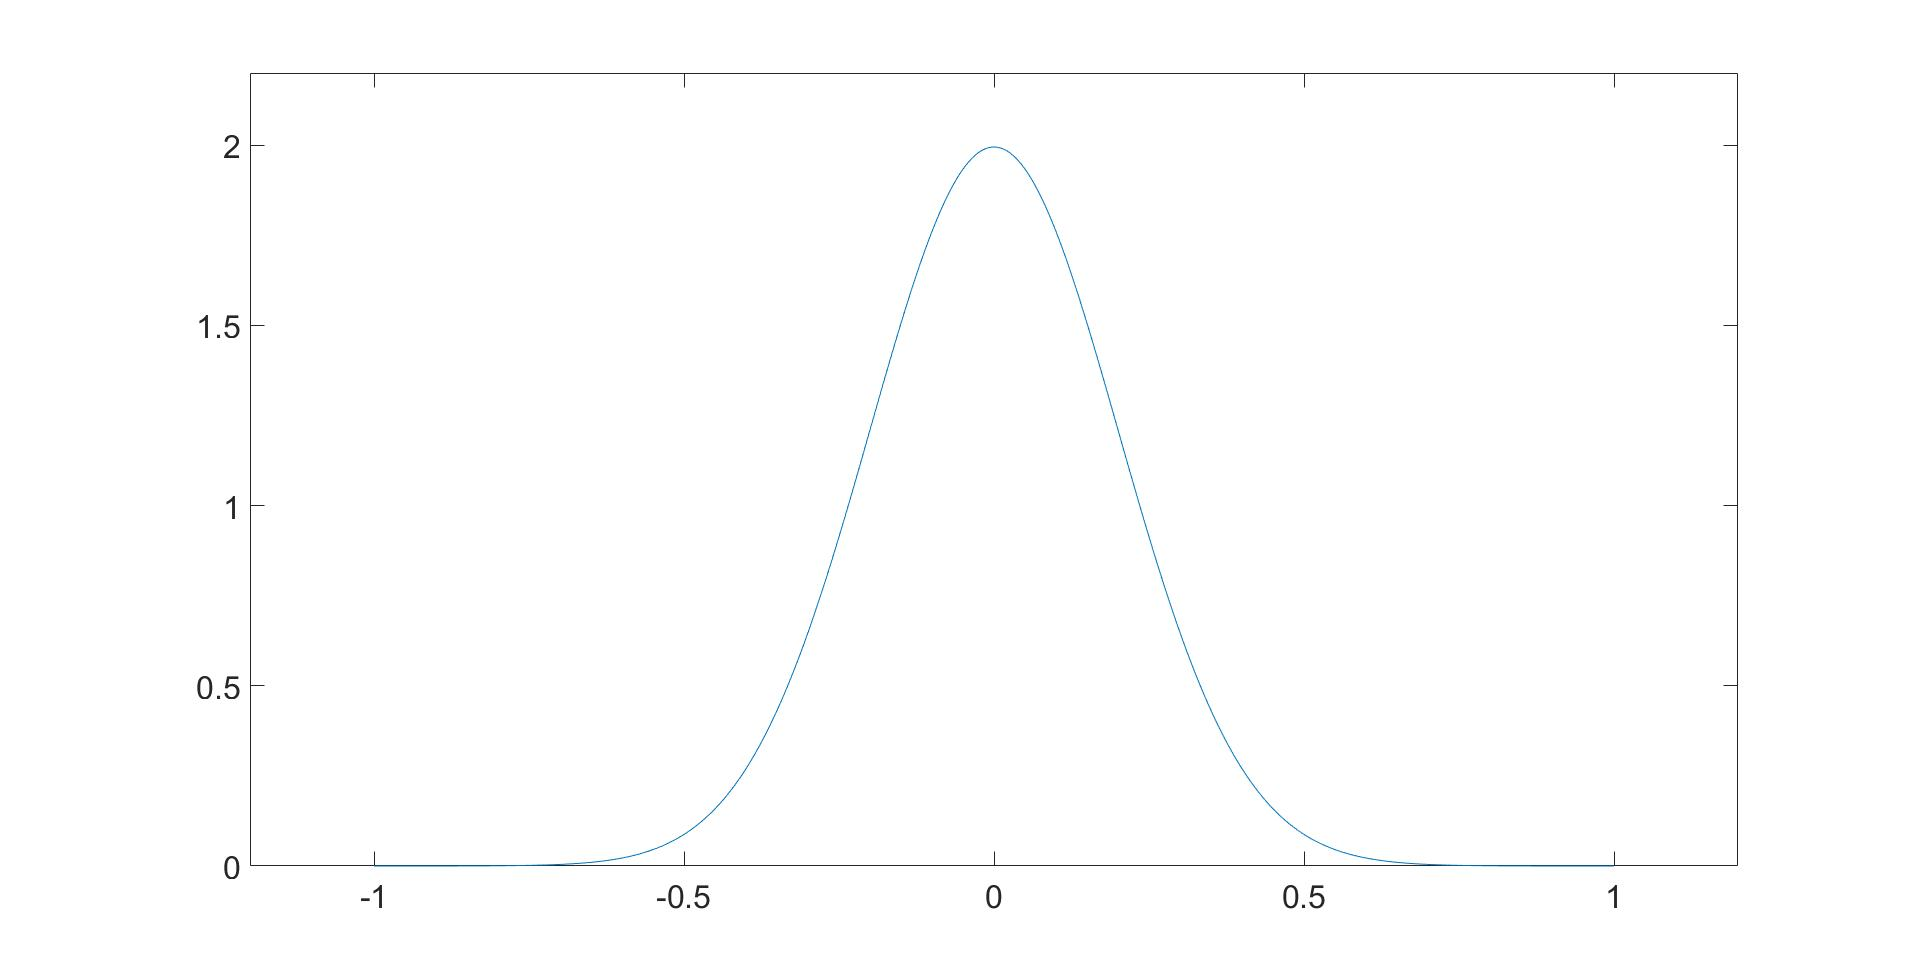
\includegraphics[width=450pt]{bellcurve}
    \caption{The Gaussian Function in 2D with $\mu$=0, $\sigma$=0.2 and $A$ = 2.}
    \label{fig:gauss}
  \end{figure}

  \begin{figure}[H]
    \centering
    \centering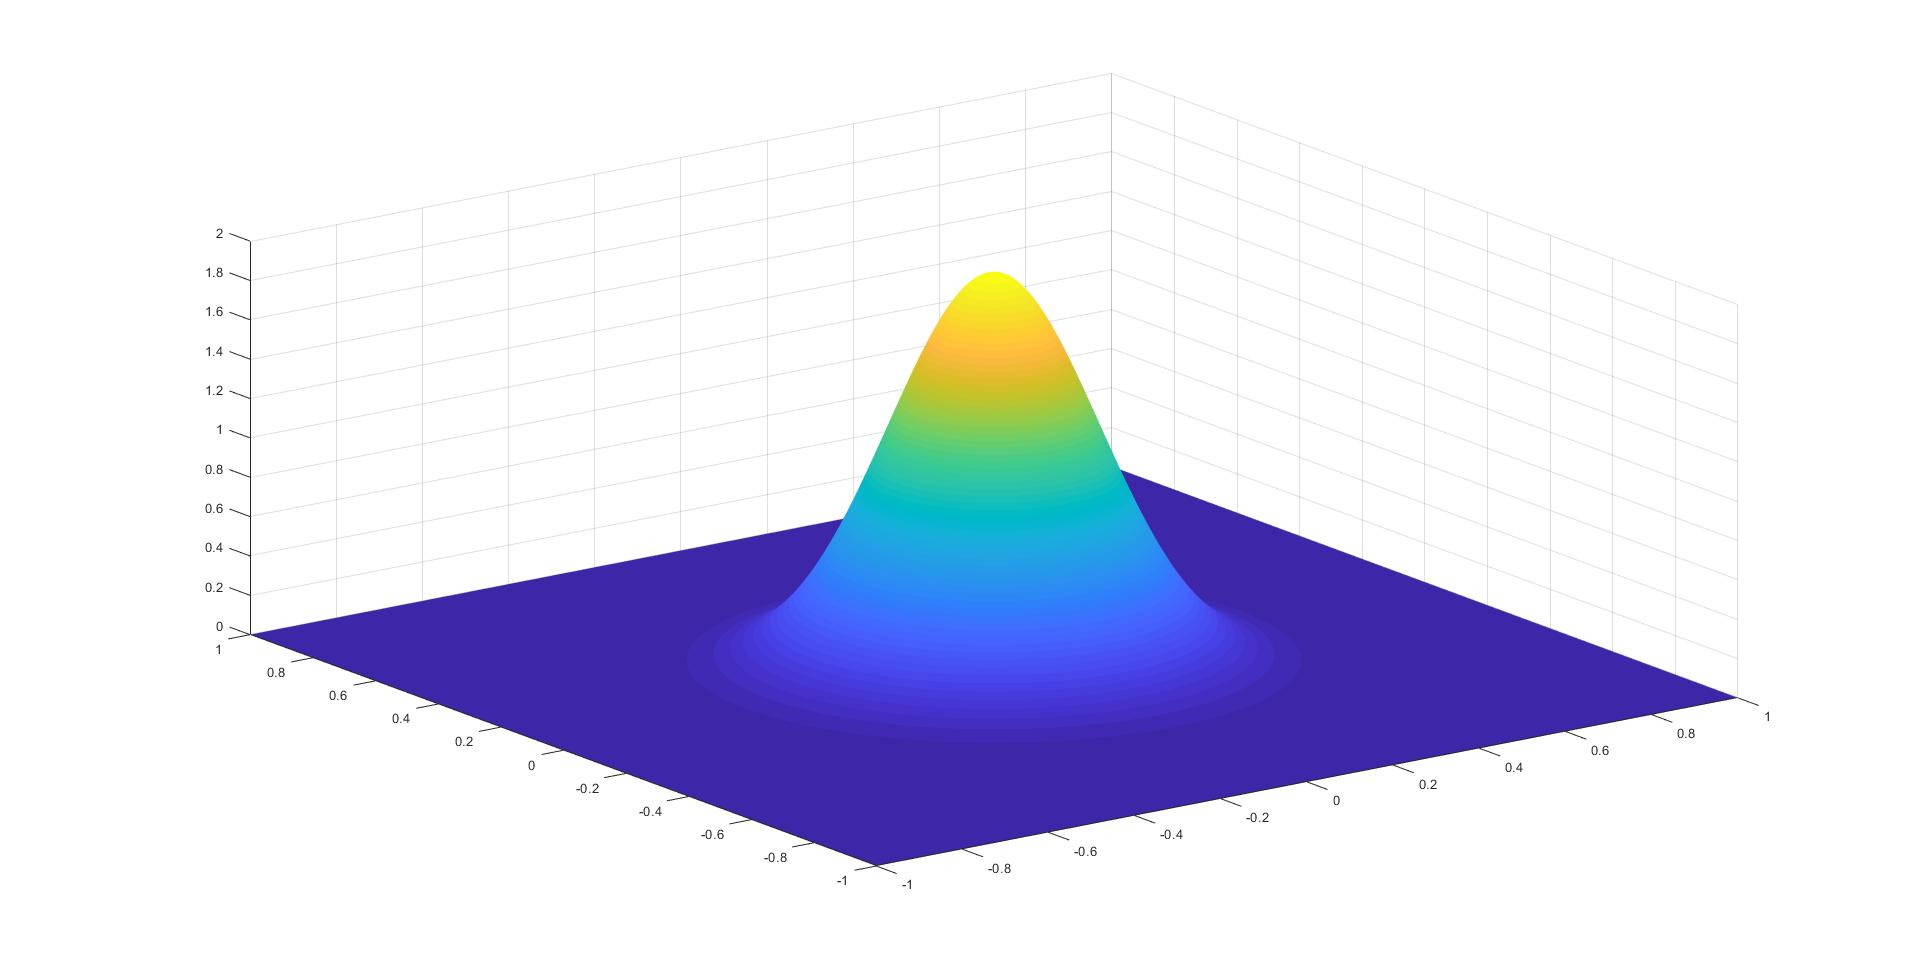
\includegraphics[width=300pt]{gauss2D}
    \caption{The Gaussian Function in 1D with $\mu$=0, $\sigma$=0.2 and $A$ = 2.}
    \label{fig:gausssurf}
  \end{figure}

  The Gaussian provides a consistent model for normal distributions, aka the bell curve. Normal distributions follow the \emph{central limit theorem} where in if a histogram is taken of a sufficiently large number of independent random variable they will distribute with a central most probable value and symmetrically fall away either side of this value. Many datasets follow this trend closely enough that the Gaussian can be used to approximate a probability distribution for them. 
  
  The general one dimensional Gaussian is described:  

\begin{equation}
    f(x) = \frac{A}{\sigma\sqrt{2\pi}}e^{-\frac{1}{2}(\frac{x-\mu}{\sigma})^2}
\label{eq:gauss}
\end{equation}

  The mean value, the central limit, of the sample distribution is $\mu$. $\sigma$ is the standard deviation or spread of the distribution, the greater the standard deviation the fatter the distribution. The amplitude $A$ is the probability for a given value in the domain. In Figure \ref{fig:gauss}, for example, the proability of a value being 0 is 2. Generally, the curve is used to determine a sample's probability desnity within a value range. This is calculated as the area under the curve using integration, generally expressed:
  
\begin{equation}
    P(x) = \int_{a}^{b}\frac{A}{\sigma\sqrt{2\pi}}e^{-\frac{1}{2}(\frac{x-\mu}{\sigma})^2}dx
    \label{eq:gausseg}
\end{equation}

In reality data sets can have many dimensions and distributions need to be able to express all of them. The notation for a multi-variate Gaussian distribution, for a k-dimensional random vector $ \bm{X} = (X_1,\hdots,X_k)^T$, is

\begin{equation}
    \bm{X} \sim \mathcal{N}_k(\mu,\,\sigma^{2})
\label{eq:multigauss}
\end{equation}






  
  
